\documentclass{article}

\usepackage[fleqn]{amsmath}
\usepackage{amssymb}
\usepackage{hyperref}
\usepackage{url}
\usepackage{graphicx}
\usepackage{geometry}
\usepackage[italian]{babel}
\usepackage{enumitem}
\usepackage{parskip}
\usepackage{chemfig}
\usepackage{pdfpages}
\usepackage{pgfplots}
\pgfplotsset{compat=1.17}
\usepackage{xcolor}
\usepackage{tikz}
\usepackage{fancybox}
\usepackage{makecell}
\usepackage{soul}
\usepackage{ulem}
\usepackage{wrapfig}
\usepackage{subcaption}
\usepackage{svg}

\usetikzlibrary{shapes.geometric, arrows}
\usetikzlibrary{decorations.pathreplacing}
\usetikzlibrary{arrows.meta}

\geometry{    
    a4paper,    
    total={170mm, 257mm},    
    left=20mm,    
    top=20mm
}
\hypersetup{    
    colorlinks=true,    
    linkcolor=black,    
    urlcolor=blue,    
    pdftitle={Chimica}
}

% === COMMANDS ===
\newcommand{\figbox}[1]{ 
    \begin{figure*}[h!]        
        \begin{center}            
            \fbox{#1}        
        \end{center}    
    \end{figure*}
}

\newcommand*\circled[1]{
    \tikz[baseline=(char.base)]{            
        \node[shape=circle,draw,inner sep=1.1pt] (char) {#1};
    }
}

\newcommand\hr{\vspace{0.1cm}\par\vspace{-.5\ht\strutbox}\noindent\hrulefill\par\vspace{0.1cm}}

% Fill the remaining space of a wrapfigure
\newcommand{\wrapfill}{
    \par
    \ifnum \value{WF@wrappedlines} > 0
        \addtocounter{WF@wrappedlines}{-1}%
        \null\vspace{
            \arabic{WF@wrappedlines}
            \baselineskip
        }
        \WFclear
    \fi
    \phantom{}
}

% === TEXT ===

\title{\textbf{Geografia economica\\Passerella 23-24}}
\author{Matteo Frongillo}

\begin{document}

\maketitle
\tableofcontents

\newpage

\section{Il tempo e la storia del pianeta Terra}
\subsection{Il tempo}
\subsubsection{Importanza del fattore tempo}
Il tempo è cruciale per comprendere molti fenomeni naturali. Ad esempio, l'erosione di una gola
da parte di un fiume avviene su una scala temporale di centinaia, migliaia o milioni di anni.

\subsubsection{Limitazioni delle misurazioni temporali umane}
\begin{itemize}
    \item Le misure temporali umane dirette vanno da frazioni di secondo a poche decine di anni;
    \item Alcuni fenomeni naturali, come movimenti delle masse d'aria e acqua e le variazioni
        climatiche stagionali, rientrano in questo intervallo di tempo.
\end{itemize}

\subsubsection{Durata di processi geologici}
Molti procesi geologici si estendono su scale temporali molto superiori alla vita umana.
Ad esempio, la formazione di uno spessore di pochi decimetri di fango sul fondale marino può
richiedere decine di migliaia di anni.

\subsubsection{Geologia e tempo}
\begin{itemize}
    \item La geologia studia la storia della Terra, la composizione della crosta terrestre e i
        processi di formazione delle rocce;
    \item Per comprendere i fenomeni geologici, è essenziale considerare il fattore tempo.
\end{itemize}

\subsubsection{Età della Terra}
\begin{itemize}
    \item La Terra ha un'età stimata di 4.54 miliardi di anni;
    \item Questa vasta scala temporale è fondamentale per comprendere fenomeni geologici come
        l'erosione fluviale e il sollevamento di catene montuose.
\end{itemize}

\begin{figure*}[ht!]
    \begin{center}
        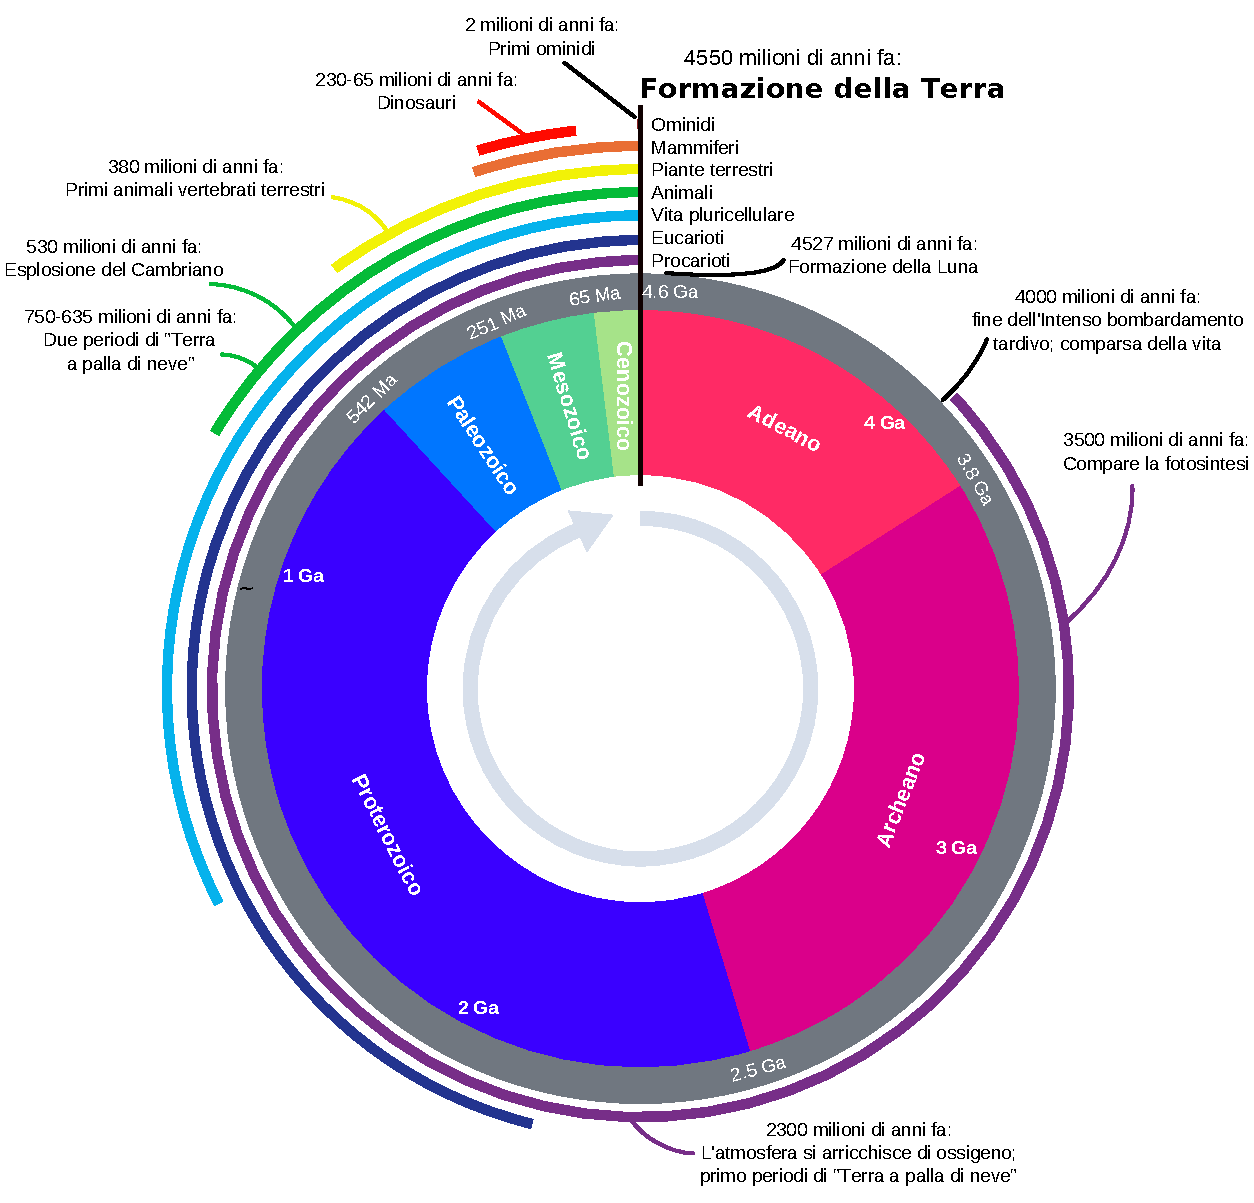
\includegraphics[width=.7\textwidth]{media/geo_fisica/Geologic_Clock_with_events_and_periods_it.pdf}
    \end{center}
\end{figure*}

\newpage
\section{La Terra come sistema}
\subsection{Il geosistema clima}
\begin{itemize}
    \item \textbf{Atmosfera:} involucro aeriforme che si estende dalla superficie del globo
        terracqueo fino a un’altezza di oltre 100 km;
    \item \textbf{Idrosfera:} insieme delle acque presenti sulla Terra in qualsiasi stato di
        aggregazione (oceani, mari, fiumi, acque sotterranee, …);
    \item \textbf{Litosfera:} involucro esterno, roccioso e rigido della Terra il quale
        comprende la crosta e la parte superiore del mantello, fino a una profondità media di
        circa 100 km;
    \item \textbf{Biosfera:} la componente vivente che comprende tutti gli organismi che vivono
        sulle terre emerse, in mare e nell’atmosfera;
    \item \textbf{Criosfera:} insieme dei ghiacci delle calotte glaciali, dei ghiacciai di
        montagna, del terreno e dei mari polari, oltre alla neve;
\end{itemize}
\phantom{}\\
\underline{Tutte le sfere interagiscono tra di loro e il sistema di sfere sfrutta e produce
energia e massa}:
\begin{itemize}
    \item Energia in entrata: radiazione solare;
    \item Energia in uscita: radiazione termica;
    \item Massa in entrata: corpo celeste che arriva sulla Terra (es. meteorite);
    \item Massa in uscita: corpo composto da elementi terrestri che lascia l'atmosfera
        (es. satellite artificiale).
\end{itemize}

\subsubsection{Processi delle placche}
\begin{itemize}
    \item \textbf{Processi esogeni:} processi attivati dall'energia solare che avvengono sulla
        superficie terrestre (es. movimenti delle acque, cambiamenti di stato e fenomeni
        meteorologici);
    \item \textbf{Processi endogeni:} processi attivati dal calore interno della Terra che
        portano alla formazione di catene montuose, terremoti e vulcani, oltre alla creazione
        e modifica dei bacini oceanici.
\end{itemize}

\subsection{Il geosistema tettonica delle placche}
\begin{figure*}[ht!]
    \begin{center}
        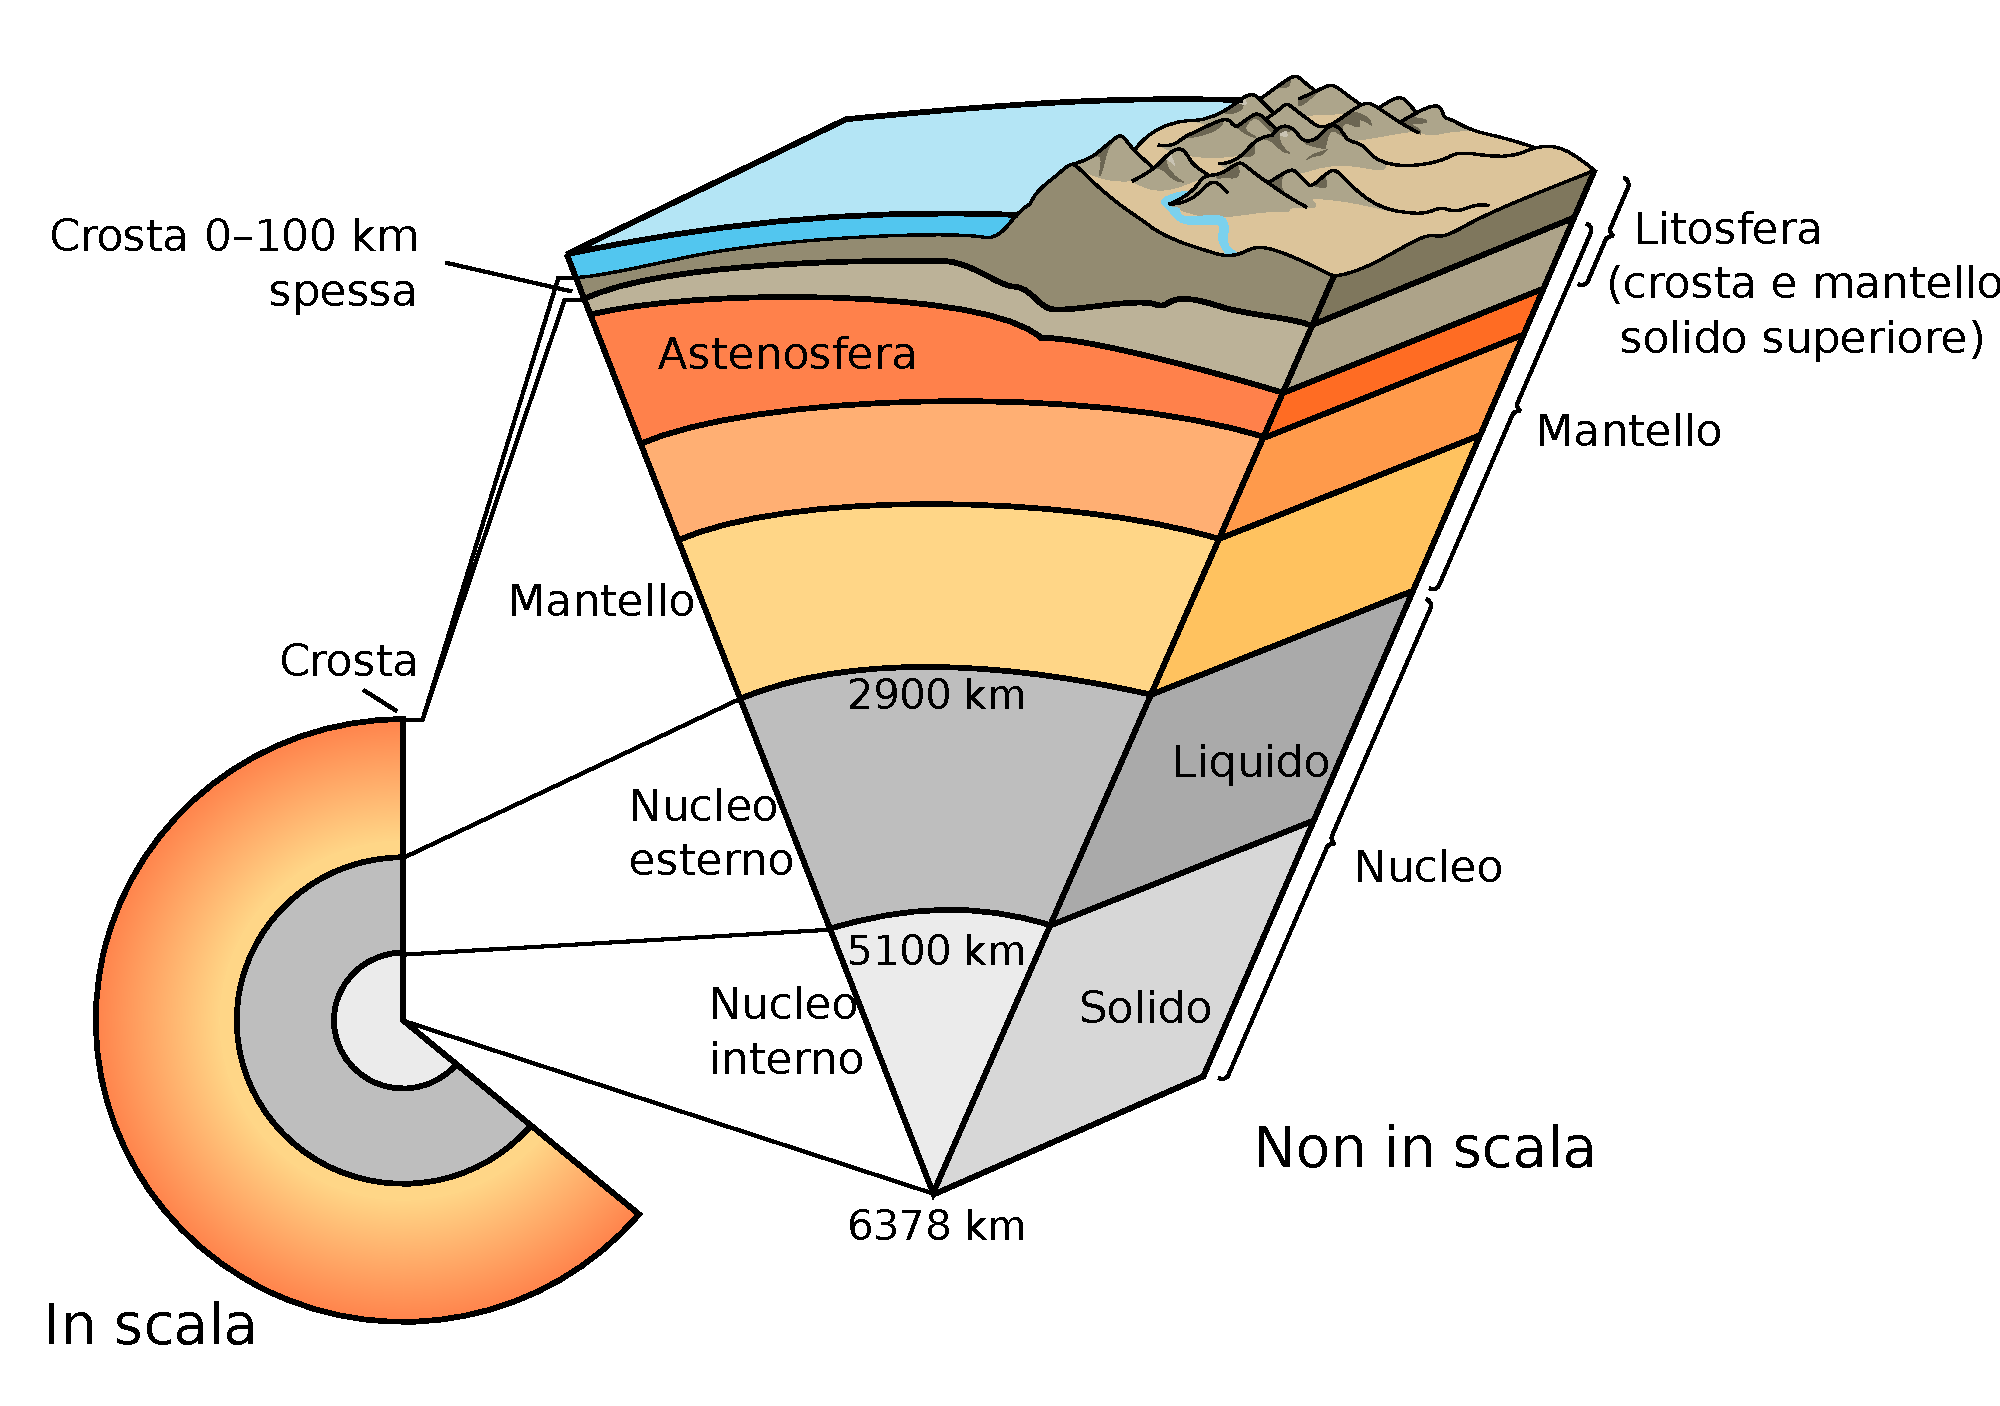
\includegraphics[width=.8\textwidth]{media/geo_fisica/Earth_cutaway_schematic-it.pdf}
    \end{center}
\end{figure*}

\newpage
\textbf{Litosfera:}

La litosfera è la parte solida e rigida della Terra che comprende la crosta terrestre
e la parte superiore del mantello. Essa è meno densa rispetto agli strati sottostanti e
si trova sopra l'astenosfera, che è più plastica e duttile.

\textbf{Astenosfera:}
\begin{itemize}
    \item L'astenosfera si trova immediatamente sotto la litosfera ed è uno strato del mantello
        superiore caratterizzato da un comportamento reologico plastico. In questo strato, la
        velocità delle onde sismiche si riduce considerevolmente.
    \item Gli spostamenti delle placche creano fenomeni magmatici che producono nuova litosfera
        e attività sismiche che sostituiscono la litosfera attuale;
    \item Poiché le onde S non si annullano completamente nell'astenosfera, i geologi ritengono
        che essa sia composta da materiali che si comportano in modo viscoelastico, permettendo
        loro di deformarsi lentamente sotto l'effetto di stress prolungati.
        \begin{itemize}
            \item Le onde S sono un tipo di onde sismiche che si propagano perpendicolarmente
                alla direzione di propagazione, causando il movimento delle particelle del
                terreno in direzioni ortogonali. Le onde S non possono propagarsi nel fluidi,
                il che significa che la loro presenza e velocità possono fornire informazioni
                sulla composizione e lo strato dei materiali che attraversano.
        \end{itemize}
\end{itemize}

\textbf{Mantello profondo:}

Porzione del mantello al di sotto dell'astenosfera il quale si estende da una profondità di
circa 400km fino al limite nucleo-mantello (profondità di 2900km).

\subsection{La tettotica delle placche}
\subsubsection{Litosfera e placche}
La litosfera è suddivisa in placche di dimensioni variabili, che si incastrano tra loro come
tessere di un mosaico, senza lasciare spazi vuoti. Le placche litosferiche sono rigide, hanno
uno spessore variabile e si muovono sull'astenosfera, che si comporta come uno strato plastico.
In questo strato, si verificano lenti movimenti di materiale con correnti ascensionali e
discensionali, noti come movimenti convettivi.

\begin{figure*}[ht!]
    \begin{center}
        \begin{tikzpicture}
            \node[anchor=south west,inner sep=0] (image) at (0,0) {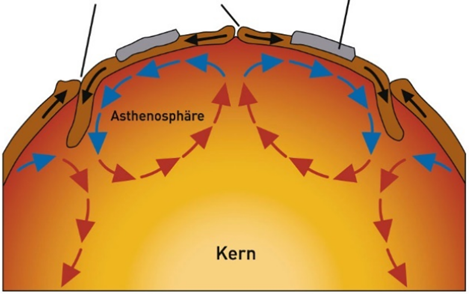
\includegraphics[width=0.4\textwidth]{media/geo_fisica/placche_tettoniche.png}};
            \node at (.4,4.5) {\footnotesize Attività sismiche};
            \node at (3.3,4.5) {\footnotesize Fenomeni magmatici};
            \node at (5.7,4.5) {\footnotesize Continenti};
        \end{tikzpicture}
    \end{center}
\end{figure*}

\subsubsection{Movimento delle placche}
Le placche si muovono orizzontalmente. Poiché sono a diretto contatto tra loro, ogni movimento
di una placca influenza quelli delle placche vicine. Questo genera instabilità lungo i margini
delle placche, mentre le regioni centrali di ciascuna placca sono sostanzialmente inattive e
stabili. Questo fenomeno permette di identificare i margini delle placche, che corrispondono a
fasce sottili e allungate caratterizzate da attività sismica.

\newpage
\subsubsection{Tipi di margini delle placche}
\setlength{\intextsep}{0pt}%
\begin{wrapfigure}{l}{.4\textwidth}
    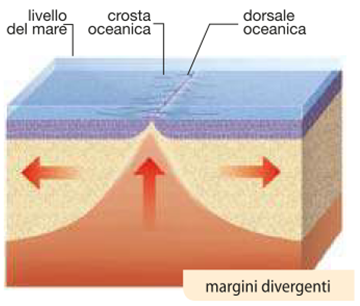
\includegraphics[width=.4\textwidth]{media/geo_fisica/margine_divergente.png}
    \vspace{-2.1cm}
\end{wrapfigure}

\phantom{}

\phantom{}

\textbf{Margini divergenti}

Sono aree in cui si crea nuova litosfera oceanica. Coincidono con le dorsali oceaniche,
ma includono anche i rift continentali, come la regione delle grandi fosse tettoniche
africane. Le due placche ai lati della dorsale si accrescono, poiché si forma un nuovo
fondale oceanico. La litosfera prodotta viene spinta lateralmente, con un moto
divergente ripetto alla dorsale. Sono caratterizzati da un'intensa
attività vulcanica e da una debole attività sismica.
\wrapfill

\setlength{\intextsep}{0pt}%
\begin{wrapfigure}{r}{.55\textwidth}
    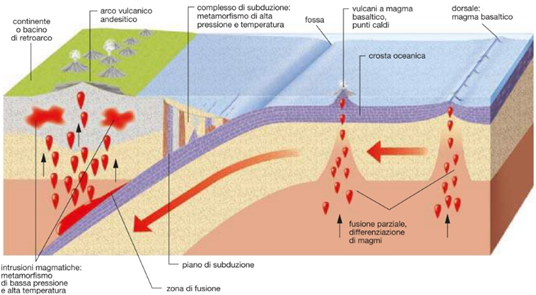
\includegraphics[width=.55\textwidth]{media/geo_fisica/margine_convergente.png}
    \vspace{-1.9cm}
\end{wrapfigure}

\phantom{}

\phantom{}

\textbf{Margini convergenti}

Lungo questi margini, le placche contigue sono sospinte l'una contro l'altra.
Coincidono con le catene montuose recenti e sono caratterizzati da fenomeni sismici
molto violenti e da un'intensa attività magmatica, sia effusiva sia intrusiva.
\wrapfill

\setlength{\intextsep}{0pt}%
\begin{wrapfigure}{l}{.45\textwidth}
    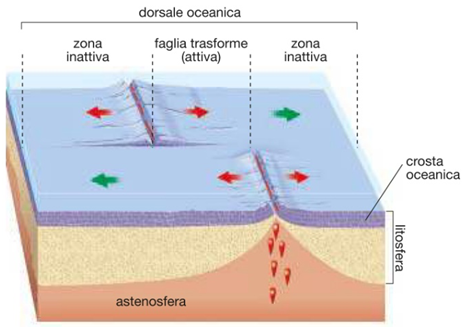
\includegraphics[width=.45\textwidth]{media/geo_fisica/margine_conservativo.png}
    \vspace{-1.9cm}
\end{wrapfigure}

\phantom{}

\textbf{Margini trasformi (o conservativi)}

Lungo questi margini, le placche scivolano l'una accanto all'altra, muovendosi in
direzioni opposte o a velocità differenti. Coincidono con faglie trasformi e sono
caratterizzati da una forte attività sismica, ma generalmente privi di attività
vulcanica o magmatica.
\wrapfill

\subsubsection{Margini divergenti}
\begin{itemize}
    \item La litosfera si incarca e si frattura, permettendo la risalita del magma
        dall'astenosfera, che solidifica formando nuova crosta oceanica. La lava basaltica
        fuoriesce, raffreddandosi e ostruendo la frattura, che viene riaperta dalla tensione
        delle correnti del mantello;
    \item Le dorsali oceaniche espandono il fondale marino a velocità variabili, formando
        nuova crosta che si allontana dalla dorsale. Questo processo crea oceani in diverse
        fasi evolutive, dal rift embrionali come la Rift Valley africana agli oceani maturi
        come l'Atlantico.
\end{itemize}

\subsubsection{Margini convergenti}
L'orogenesi avviene ai margini convergenti delle placche tettoniche, dove la collisione tra
placche causa piegamenti e sovrascorrimenti che formano le montagne. Questo processo include la
subduzione e la collisione continentale, creando catene montuose come l'Himalaya e le Alpi.
\begin{itemize}
    \item I margini convergenti sono i confini tra placche tettoniche dove avviene la collisione.
        Esistono quattro tipi di convergenza:
        \begin{enumerate}
            \item Litosfera continentale vs. oceanica: la placca oceanica subduce sotto quella
                continentale, formando una fossa oceanica e un arco vulcanico, con intensa
                attività sismica (es. Ande);
            \item Litosfera oceanica vs. oceanica: una placca subduce sotto l'altra, formando
                una fossa oceanica e un arco vulcanico insulare (es. Giappone, Filippine);
            \item Litosfera continentale vs. continentale: nessuna placca subduce, si formano
                catene montuose tramite piegamenti e sovrascorrimenti (es. Himalaya, Alpi);
            \item Placca mista vs. oceanica: la litosfera oceanica subduce, mentre quella
                continentale causa terremoti e deformazioni (es. margine tra placca
                euroasiatica e africana).
        \end{enumerate}
\end{itemize}

\subsubsection{Margini conservativi}
\begin{itemize}
    \item I margini conservativi sono caratterizzati dallo scorrimento orizzontale delle placche
        tettoniche senza creare o distruggere litosfera. Le placche si muovono lateralmente
        lungo faglie trasformi, causando terremoti violenti ma senza formazione di montagne o
        vulcani significativi (es. Faglia di San Andreas);
    \item Le faglie trasformi nelle dorsali oceaniche interrompono la continuità delle dorsali,
        con movimenti opposti dei blocchi rocciosi, generando terremoti dovuti alla diversa
        velocità di espansione.
\end{itemize}

\subsubsection{Teoria della tettonica delle placche}
La teoria è supportata da numerose evidenze e da due punti chiave:
\begin{enumerate}
    \item La litosfera è divisa dall'astenosfera, con movimenti convettivi;
    \item Le placche sono soggette a forze ai loro margini o sotto la loro superficie basale.
        La causa principale dei movimenti delle placche sono i movimenti convettivi del mantello.
\end{enumerate}

\section{Terremoti e vulcani}
\subsection{Terremoti}
\begin{figure*}[ht!]
    \begin{center}
        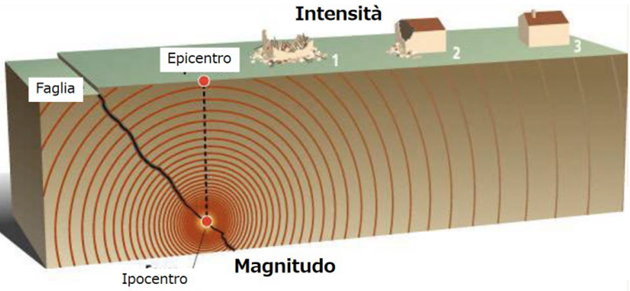
\includegraphics[width=.6\textwidth]{media/geo_fisica/terremoti.png}
    \end{center}
\end{figure*}

\subsubsection{Definizioni}
\begin{itemize}
    \item \textbf{Epicentro}: Punto sulla superficie terrestre direttamente sopra l'ipocentro;
    \item \textbf{Ipocentro}: Punto sotterraneo dove ha origine il terremoto, anche detto focus;
    \item \textbf{Faglia}: Frattura nella crosta terrestre lungo la quale avviene il movimento
        delle placche;
    \item \textbf{Magnitudo}: Misura dell'energia rilasciata da un terremoto, quantificata con
        la scala Richter;
    \item \textbf{Intensità}: Misura degli effetti di un terremoto sulla superficie terrestre,
        valutata con la scala Mercalli;
\end{itemize}

\subsubsection{Tipi di onde sismiche}
\begin{itemize}
    \item Onde P (primarie, compressionali): onde di compressione che viaggiano più velocemente
        e sono le prime ad rilevate da un sismografo;
    \item Onde S (secondarie, di taglio): onde di taglio che viaggiano più lentamente e vengono
        rilevate successivalemten;
    \item Onde superficiali: onde che viaggiano lungo la superficie terrestre, principali
        cause della maggior parte dei danni durante un terremoto.
\end{itemize}

\subsubsection{Scale di misurazione}
\begin{itemize}
    \item \textbf{Scala Mercalli}: Scala che misura l'intensità dei terremoti in base agli
        effetti osservati e si basa sui danni materiali, dunque dipende dalla distanza
        dall'epicentro. È divisa in 12 gradi: I (impercepibile) a XII (distruttivo);
    \item \textbf{Scala Richter}: Scala logaritmica che misura la magnitudo (energia e forza)
        di un terremoto, ogni aumento di un'unità corrisponde a un aumento di dieci volte
        nell'ampiezza delle onde sismiche, dunque non dipende dalla distanza dall'epicentro.
\end{itemize}

\subsubsection{Strumenti di misurazione e prevenzione}
\begin{itemize}
    \item \textbf{Sismogramma}: Grafico registrato da un sismografo che mostra le onde sismiche
        generate dal terremoto;
\begin{figure*}[ht!]
    \begin{center}
        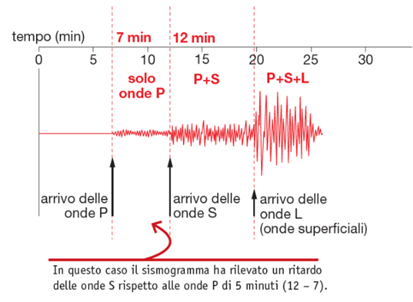
\includegraphics[width=.4\textwidth]{media/geo_fisica/simsogramma.png}
    \end{center}
\end{figure*}

    \item \textbf{Previsione dei terremoti}: Attualmente difficile da realizzare con precisione,
        si basa su studi statistici e storici delle aree sismiche;
    \item \textbf{Rischio sismico}: Valutazione della probabilità di occorrenza e dell'impatto
        potenziale di un terremoto in una determinata area;
    \item \textbf{Misure di sicurezza}: Costruzioni antisismiche, piani di evacuazione e sistemi
        di allerta precoce sono fondamentali per ridurre i danni e salvare vite umane.
\end{itemize}

\subsection{Vulcani}
\subsubsection{Forma}
\begin{itemize}
    \item \textbf{Forma dei vulcani}: Include coni stratificati, scudi, caldere e vulcani a cono
        di scorie;
    \item \textbf{Coni stratificati}: Vulcani con eruzioni esplosive e struttura a strati di
        lava e cenere (es. Monte Fuji, Vesuvio);
    \item \textbf{Vulcani a scudo}: Vulcani con eruzioni effusive e una forma larga e bassa
        (es. Mauna Loa, Mauna Kea).
\end{itemize}

\subsubsection{Tipi di eruzione}
\begin{itemize}
    \item \textbf{Eruzioni esplosive}: Emissioni violente di gas, cenere e frammenti solidi,
        tipiche dei vulcani a cono stratificato;
    \item \textbf{Eruzioni effusive}: Colate laviche relativamente tranquille, comuni nei
        vulcani a scudo.
\end{itemize}
    
\subsubsection{Creazione}
\begin{itemize}
    \item \textbf{Caldera}: Grande cratere formatosi per il collasso della camera magmatica dopo
        un'eruzione (es. Yellowstone, Crater Lake);
    \item \textbf{Vulcani a cono di scorie}: Piccoli vulcani con eruzioni esplosive di breve
        durata che formano coni di scorie (es. Parícutin).
\end{itemize}
    
\subsubsection{Elementi}
\begin{itemize}
    \item \textbf{Camera magmatica}: Riserva sotterranea di magma che alimenta i vulcani;
    \item \textbf{Fumarole}: Aperture nei vulcani da cui fuoriescono gas;
    \item \textbf{Lava}: Magma che raggiunge la superficie terrestre durante un'eruzione;
    \item \textbf{Cenere vulcanica}: Particelle fini di materiale piroclastico espulse durante
        un'eruzione esplosiva;
    \item \textbf{Gas vulcanici}: Principalmente vapore acqueo, anidride carbonica e diossido
        di zolfo, possono influenzare il clima;
    \item \textbf{Hotspot}: Punti caldi nel mantello che causano attività vulcanica lontano dai
        margini delle placche (es. Hawaii, Islanda).
\end{itemize}
    
\subsubsection{Prevenzione}
\begin{itemize}
    \item \textbf{Previsione delle eruzioni}: Basata su monitoraggio di segnali precursori come
        aumento della sismicità, deformazioni del terreno e variazioni nei gas vulcanici;
    \item \textbf{Rischio vulcanico}: Valutazione della probabilità di eruzioni vulcaniche e del
        loro impatto potenziale su persone, infrastrutture e ambiente;
    \item \textbf{Misure di sicurezza}: Evacuazioni, piani di emergenza e monitoraggio costante
        dei vulcani attivi sono cruciali per mitigare i rischi associati alle eruzioni.
\end{itemize}

\newpage
\section{Rocce, geomorfologia e suolo}

\subsection{Processi endogeni e esogeni}

\subsubsection{Processi endogeni}
I processi endogeni derivano dal calore della Terra. Alcuni esempi:
\begin{itemize}
    \item Diastrofismo (Tettonica delle placche);
    \item Riorganizzazione crostale (Terremoti);
    \item Vulcanismo.
\end{itemize}

\subsubsection{Processi esogeni}
I processi esogeni derivano dai processi endogeni e sono inversamente proporzionali ad essi:
\begin{itemize}
    \item Agiscono appena si comincia a formare un rilievo;
    \item Contrastano l'azione dei processi endogeni.
\end{itemize}
\vspace*{.3cm}
\begin{figure*}[ht!]
    \begin{center}
        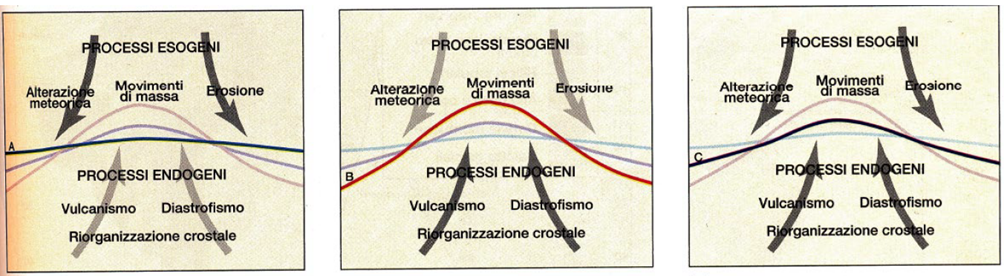
\includegraphics[width=\textwidth]{media/geo_fisica/processi_geo.png}
    \end{center}
\end{figure*}
\phantom{}

\subsection{Le rocce}
I processi che portano alla creazione delle rocce sono tre:
\begin{itemize}
    \item Processo magmatico, ossia la solidificazione del magma:
    \begin{itemize}
        \item Rocce magmatiche effusive;
        \item Rocce magmatiche intrusive;
    \end{itemize}
    \item Processo sedimentario: avviene sulla superficie terrestre;
    \item Processo metamorfico: avviene all'interno della crosta terrestre.
\end{itemize}

\subsubsection{Rocce magmatiche effusive}
Si formano quando la lava, a contatto con l'aria o l'acqua, si raffredda velocemente.

\subsubsection{Rocce magmatiche intrusive}
Si formano quando il magma non riesce ad emergere in superficie e rimane intrappolato tra le
rocce in bolle o filoni magmatici, nei quali si raffredda lentamente.

\subsubsection{Rocce sedimentarie}
Si formano quando altri tipi di rocce sono esposte sulla superficie terrestre e vengono
disgregate dall'azione degli \textbf{agenti esogeni} dell'atmosfera (piogge), dell'idrosfera
(fiumi, esondazioni) e della biosfera (funghi, batteri, piante). Queste interazioni possono
durare milioni di anni e possono essere descritte in tappe:
\begin{itemize}
    \item \textbf{Degradazione}
    \begin{itemize}
        \item Disgregazione fisica (es. frane, crio/termoclastismo);
        \item Alterazione chimica (es. idrolisi, ossidazione);
    \end{itemize}
    \item \textbf{Sedimentazione}
    \begin{itemize}
        \item Cementificazione → Diagenesi (es. sabbia cementata);
        \item Trasporto (es. fiumi, ghiacciai);
        \item Deposizione (es. delta, foce, arginamento);
        \item Calcificazione → (es. deposizione chimica e successiva evaporazione).
    \end{itemize}
\end{itemize}

\subsubsection{Rocce metamorfiche}
Si formano quando altri tipi di rocce superficiali vengono trasportate in profondità a causa
\textbf{agenti endogeni}, come imponenti movimenti della crosta, ed entrando in contatto con
temperature e pressioni molto elevate, trasformando così la loro struttura e la loro
composizione mineralogica. Le trasformazioni metamorfiche rimangono comunque allo stato solido.
Esse possono essere suddivise in due tipi:
\begin{itemize}
    \item Rocce scistose (o regionali), quando vengono stirate dai movimenti della crosta;
    \item Rocce di contatto, quando vengono trasformate dal calore del magma vicino.
\end{itemize}

\subsubsection{Il ciclo litogenetico}
\phantom{}

\begin{figure*}[ht!]
    \begin{center}
        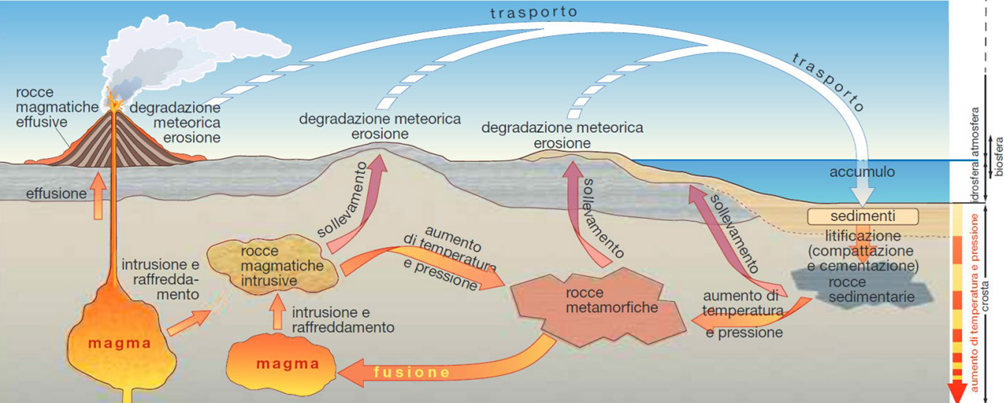
\includegraphics[width=\textwidth]{media/geo_fisica/ciclo_litogenetico.png}
    \end{center}
\end{figure*}

\newpage
\section{Il suolo}
\subsection{Materiali geologici sulla superficie del pianeta}
\begin{itemize}
    \item Roccia in posto (es. montagne);
    \item Depositi superficiali (es. rocce sedimentarie);
    \item Suolo.
\end{itemize}

\subsubsection{Il suolo}
Il suolo è lo strato incoerente di detriti minerali prodotti dal disfacimento delle rocce,
ricco di materia organica, liquidi, gas e forme di vita, che poggia sulla roccia in posto
inalterata.

\subsection{La formazione dei suoli}
\subsubsection{La struttura}
\begin{itemize}
    \item \textbf{Orizzonte A}
    \begin{itemize}
        \item Ricco di materia organica;
        \item Le acque piovane si infiltrano e trasportano verso il basso le particelle
            argillose più piccole, lasciando quelle più grandi in superficie;
    \end{itemize}
    \item \textbf{Orizzonte B}
    \begin{itemize}
        \item Povero di materia organica;
        \item Ricco di particelle argillose;
    \end{itemize}
    \item \textbf{Orizzonte C}
    \begin{itemize}
        \item Costituito da particelle di suolo e da frammenti di roccia non ancora
            completamente alterati;
        \item In questo orizzonte si ha un passaggio graduale verso la roccia madre;
    \end{itemize}
    \item \textbf{Roccia madre (R)}.
\end{itemize}

\subsubsection{I climi}
\begin{itemize}
    \item \textbf{Clima temperato}
    \begin{itemize}
        \item Il suolo è ricco di humus e adatto alla crescita di piante
    \end{itemize}
    \item \textbf{Clima caldo umido}
    \begin{itemize}
        \item Il suolo è povero di humus, ma con una vegetazione rigogliosa
    \end{itemize}
    \item \textbf{Clima arido}
    \begin{itemize}
        \item Il suolo è povero di humus, con vegetazione bassa e rada
    \end{itemize}
\end{itemize}
\phantom{}

\begin{figure*}[ht!]
    \begin{center}
        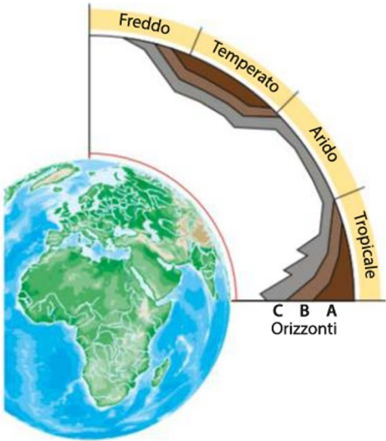
\includegraphics[width=.35\textwidth]{media/geo_fisica/profili_terra.png}
    \end{center}
\end{figure*}

\subsubsection{La formazione del suolo}
\begin{itemize}
    \item La roccia madre fornisce il detrito e determina la composizione della parte minerale;
    \item La pendenza del terreno incide in modo rilevante sullo spessore del suolo;
    \item Se la pendenza è molto forte, il suolo può essere del tutto assente, come sulle pareti
        rocciose di alta montagna;
    \item Il clima influisce sui processi di formazione, sullo spessore del suolo e sullo
        sviluppo e sul tipo di vegetazione.
\end{itemize}

\newpage
\section{I moti di rotazione e rivoluzione}
\subsection{Le conseguenze dei moti}

\subsubsection{Forza centrifuga}
Con il moto di \textbf{rotazione} della Terra si hanno due tipi di velocità e di forze:
\begin{itemize}
    \item Velocità di rotazione lineare e angolare;
    \item Forza centrifuga e centripeta.
\end{itemize}

\subsubsection{Ciclo giorno-notte}
La \textbf{rotazione} della Terra fa sì che ci sia ciclicamente il dì e la notte.

\subsubsection{Stagioni}
La \textbf{rivoluzione} della Terra attorno al Sole fa sì che il proprio asse rotei
periodicamente attorno al centro di massa terrestre, comportando così l'alternanza tra le
stagioni.

\subsubsection{Forza di Coriolis}
I corpi in volo, a causa dell'asse di rotazione, non vengono spostati in linea d'aria.
\begin{itemize}
    \item Nell'emisfero nord i corpi si spostano verso destra.
    \item Nell'emisfero sud i corpi si spostano verso sinistra.
\end{itemize}
\phantom{}

\begin{center}
    \begin{tikzpicture}
        % Diagramma Polo Nord
        \draw[thick] (0,2) -- (6,2);
        \draw[->, red, thick] (3,2) .. controls (2.5,1.5) .. (2,1.5);
        \draw[->, black, thick] (3,2) -- (3,1.25);
        \node[right] at (6,2) {Polo Nord ($V_{min}$)};
        
        % Diagramma Equatore
        \draw[thick] (0,0) -- (6,0);
        \draw[->, red, thick] (3,0) .. controls (3.5,-0.5) .. (4,-0.5);
        \draw[->, black, thick] (3,0) -- (3,-0.75);
        \draw[->, red, thick] (3,0) .. controls (3.5,0.5) .. (4,0.5);
        \draw[->, black, thick] (3,0) -- (3,0.75);
        \node[right] at (6,0) {Equatore ($V_{max}$)};
        
        % Diagramma Polo Sud
        \draw[thick] (0,-2) -- (6,-2);
        \draw[->, red, thick] (3,-2) .. controls (2.5,-1.5) .. (2,-1.5);
        \draw[->, black, thick] (3,-2) -- (3,-1.25);
        \node[right] at (6,-2) {Polo Sud ($V_{min}$)};
    \end{tikzpicture}
\end{center}

\subsubsection{Solstizi ed equinozi}
\begin{tabular}{|l|l|l|l|l|}
    \hline & \begin{tabular}{l} 
    Solstizio \\
    d'inverno
    \end{tabular} & \begin{tabular}{l} 
    Equinozio di \\
    primavera
    \end{tabular} & Solstizio d'estate & Equinozio d'autunno \\
    \hline Data & 22 dicembre & 21 marzo & 21 giugno & 23 settembre \\
    \hline \begin{tabular}{l} 
    Parallelo in \\
    cui il sole è \\
    allo Zenit (a \\
    mezzogiorno)
    \end{tabular} & \begin{tabular}{c} 
    Tropico del \\
    Capricorno
    \end{tabular} & Equatore & Tropico del Cancro & Equatore \\
    \hline \begin{tabular}{l} 
    Luogo con \\
    più di ore di \\
    luce
    \end{tabular} & Polo Sud & \begin{tabular}{l} 
    Stessa durata del di \\
    e della notte su \\
    tutto il pianeta
    \end{tabular} & Polo Nord & \begin{tabular}{l} 
    Stessa durata del dì \\
    e della notte su \\
    tutto il pianeta
    \end{tabular} \\
    \hline \begin{tabular}{l} 
    Luogo con \\
    meno ore di \\
    luce
    \end{tabular} & Polo Nord & \begin{tabular}{l} 
    Stessa durata del dì \\
    e della notte su \\
    tutto il pianeta
    \end{tabular} & Polo Sud & \begin{tabular}{l} 
    Stessa durata del dì \\
    e della notte su \\
    tutto il pianeta
    \end{tabular} \\
    \hline \begin{tabular}{l} 
    Che stagione \\
    inizia \\
    nell'emisfero \\
    nord
    \end{tabular} & Inverno & Primavera & Estate & Autunno \\
    \hline \begin{tabular}{l} 
    Che stagione \\
    inizia \\
    nell'emisfero \\
    sud
    \end{tabular} & Estate & Autunno & Inverno & Primavera \\
    \hline
\end{tabular}

\subsubsection{Emisferi}
\phantom{}
\begin{figure*}[ht!]
    \begin{center}
        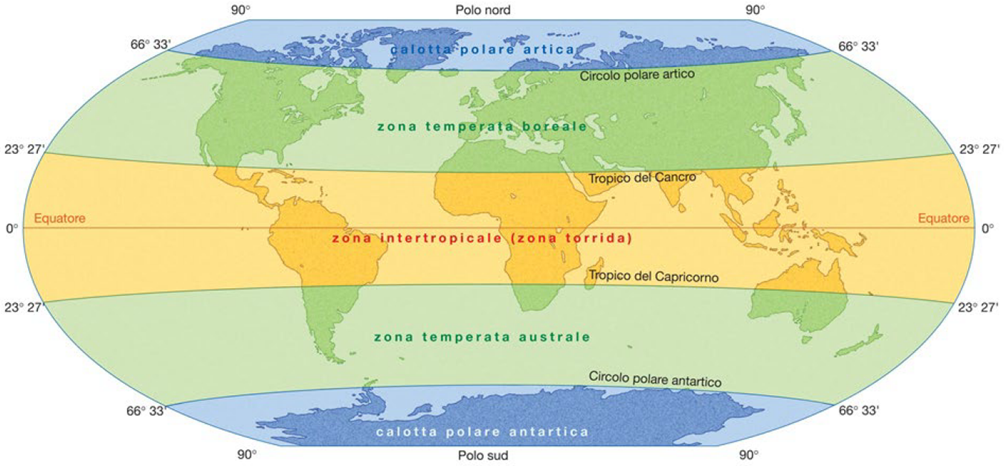
\includegraphics[width=\textwidth]{media/geo_fisica/emisferi.png}
    \end{center}
\end{figure*}
\phantom{}

\subsection{Zone climatiche}
\subsubsection{Zona intertropicale}
    \begin{itemize}
        \item Raggi solari perpendicolari alla superficie terrestre due volte all'anno.
        \item In generale l'illuminazione è sempre molto intensa.
        \item Poca differenza di durata tra il dì e la notte.
    \end{itemize}

\subsubsection{Zona temperata boreale e australe}
    \begin{itemize}
        \item I raggi del sole giungono sempre più o meno obliqui, mai perpendicolari alla superficie.
        \item Giornate corte in inverno e lunghe in estate.
    \end{itemize}

\subsubsection{Calotta polare artica e antartica}
    \begin{itemize}
        \item I raggi del sole giungono sempre molto inclinati.
        \item Si alternano un "gran dì" e una "gran notte".
    \end{itemize}

\subsection{Struttura e composizione dell'atmosfera}
\subsubsection{Composizione dell'aria}
\begin{itemize}
    \item 78.1\% Azoto (N$_2$)
    \item 20.9\% Ossigeno (O$_2$)
    \item 0.94\% Argon (Ar)
    \item 0.038\% Diossido di carbonio (CO$_2$)
\end{itemize}

\subsubsection{Gli strati dell'atmosfera}
\begin{tabular}{|l|l|l|} 
    \hline Strato & Altitudine & Fenomeni tipici \\
    \hline Esosfera & - & \begin{tabular}{l} 
    Aurore polari \\
    Riflessione onde radio
    \end{tabular} \\ \hline
    Termosfera & $500-1000 \mathrm{~km}$ & \begin{tabular}{l} 
    Aurore polari \\
    Riflessione onde radio
    \end{tabular} \\ \hline
    Mesosfera & $80 \mathrm{~km}$ & \begin{tabular}{l} 
    Nubi nottilucenti
    \end{tabular} \\ \hline
    Stratosfera & $50 \mathrm{~km}$ & Assorbimento dei raggi UV \\ \hline
    Troposfera & $7-17 \mathrm{~km}$ & Fenomeni atmosferici \\
    \hline
    \end{tabular}

\subsection{L'umidità nell'aria}

\subsubsection{Umidità assoluta}
La quantità di vapore acqueo in grammi contenuta in 1 m$^3$ di aria.

\subsubsection{Umidità massima}
La quantità massima di vapore acqueo che può contenere 1 m$^3$ di aria.

\subsubsection{Umidità relativa}
Il rapporto tra l'umidità assoluta e l'umidità massima possibile: \(UR=\frac{m_{UA}}{m_{UAmax}}\)

\subsubsection{Limite di saturazione e punto di rugiada}
La quantità massima di vapore acqueo all'interno dell'aria è dipendente dalla temperatura e
viene chiamato limite di saturazione. Quando l'umidità relativa equivale all'umidità massima,
si parla di punto di rugiada.


\subsection{La pressione atmosferica e lo sviluppo dei venti}

\subsubsection{Ciclone}
L'aria calda si scontra sul suolo e va verso l'alto, creando bassa pressione.

\subsubsection{Anticiclone}
L'aria fredda si scontra in aria e va verso il basso, creando alta pressione.

\vspace*{.8cm}

\begin{figure}[ht!]
    \centering
    \begin{minipage}{0.37\textwidth}
        \centering
        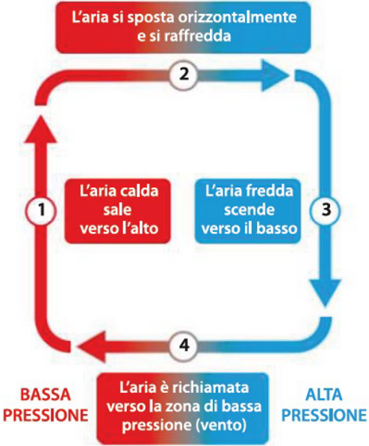
\includegraphics[width=\linewidth]{media/geo_fisica/ciclo_aria.png}
        \caption*{Cico dell'aria}
    \end{minipage}\hfill
    \begin{minipage}{0.60\textwidth}
        \centering
        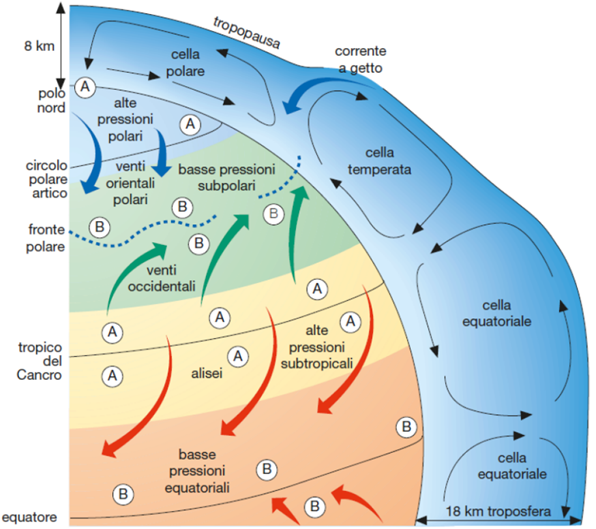
\includegraphics[width=\linewidth]{media/geo_fisica/cicloni.png}
        \caption*{Mappa dei cicloni}
    \end{minipage}
\end{figure}

\subsubsection{Inter Tropical Convergence Zone (ITCZ)}
Le principali correnti convergenti si trovano:
\begin{itemize}
    \item Ai poli Nord e Sud;
    \item Ai Tropici del Cancro e del Capricorno.
\end{itemize}

I venti divergenti dei Fronti Polari e dell'Equatore convergono alle fasce dei Tropici, creando
alta pressione sul suolo (anticiclone) e siccità.\\
I venti si spostano periodicamente poiché sono condizionati sia dalla rivoluzione della Terra
sia dal tipo di superficie sulla quale agiscono.

\subsection{Classificazione e analisi dei climi}
\subsubsection{Elementi climatici}
Gli elementi climatici sono fenomeni misurabili dell'atmosfera e descrivono il clima:
\begin{itemize}
    \item Precipitazioni;
    \item Vento;
    \item Pressione;
    \item Irradiazione solare;
    \item Temperatura;
    \item Umidità.
\end{itemize}

\subsubsection{Fattori climatici}
Determinano e influenzano il clima:
\begin{itemize}
    \item Latitudine (distanza dall'equatore);
    \item Altitudine;
    \item Continentalità (distanza dagli oceani).
\end{itemize}

\subsubsection{Classificazione di Köppen}
La classificazione di Köppen tende a dividere i climi seguendo questi punti:
\begin{itemize}
    \item Temperatura media annua;
    \item Temperatura media mensile;
    \item Precipitazioni medie annue;
    \item Precipitazioni medie mensili;
    \item Tipo di associazione vegetale.
\end{itemize}

\subsubsection{Tipi di clima}
\begin{enumerate}
    \item Clima caldo umido: Le temperature medie superano sempre i 15°C e le precipitazioni
        sono abbondanti;
    \item Clima arido: Precipitazioni scarsissime;
    \item Clima temperato: Inverni non rigidi e precipitazioni generalmente moderate;
    \item Clima freddo: I mesi freddi prevalgono, con precipitazioni moderate o scarse che si
        verificano soprattutto durante l'estate;
    \item Clima nivale: La temperatura media del mese più caldo è sempre inferiore a 10°C,
        mentre le precipitazioni (soprattutto nevose) sono scarse.
\end{enumerate}
\begin{center}
    \begin{tikzpicture}
        % Disegna i quadranti
        \draw[thick, ->] (0,0) -- (0,4);
        \draw[thick, ->] (0,0) -- (4,0);
        \draw[thick] (2,0) -- (2,4);
        \draw[thick] (0,2) -- (4,2);
    
        % Numeri nei quadranti
        \node at (1,3) {\Large 2};
        \node at (3,3) {\Large 1};
        \node at (1,1) {\Large 5};
        \node at (3,1) {\Large 3};
    
        \node at (0,4.2) {Temperatura};
        \node at (5.2,0) {Precipitazioni};
    
        \node at (-0.3,0.3) {\large -};
        \node at (-0.3,3.5) {\large+};
        \node at (0.3,-0.3) {\large -};
        \node at (3.5,-0.3) {\large+};
    \end{tikzpicture}
\end{center}
Il clima freddo (4) è difficilmente posizionabile in un grafico simile.

\newpage
\section{Cambiamento climatico e politica del clima}

\subsection{0 - Punto di partenza}

\subsubsection{Ciclo climatico}
\setlength{\intextsep}{0pt}%
\begin{wrapfigure}{r}{.6\textwidth}
    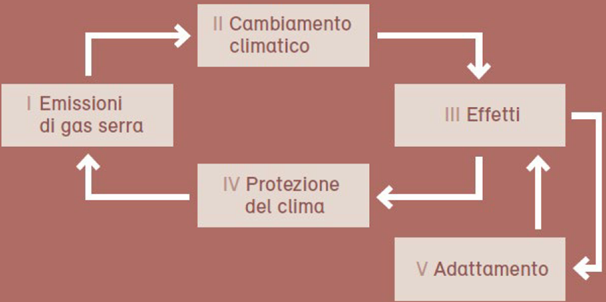
\includegraphics[width=.6\textwidth]{media/geo_fisica/ciclo_climatico.png}
    \vspace{-2.4cm}
\end{wrapfigure}

\phantom{}

\textbf{Ciclo climatico}
\begin{enumerate}
    \item Emissioni di gas serra;
    \item Cambiamento climatico;
    \item Effetti;
    \item Protezione del clima;
    \item Adattamento.
\end{enumerate}
\wrapfill


\subsection{1 - Il sistema climatico}
\subsubsection{Sfere climatiche}
\begin{itemize}
    \item Atmosfera;
    \item Idrosfera (precipitazioni, oceani, corsi d'acqua);
    \item Criosfera (calotte glaciali, ghiacciai, neve);
    \item Biosfera marittima e terrestre;
    \item Pedosfera (suoli);
    \item Crosta terrestre;
    \item Mantello terrestre.
\end{itemize}

\subsubsection{Effetto serra naturale}
L'effetto serra naturale è dato dai gas serra che bloccano il flusso retroattivo dei raggi
solari appena deviati verso l'alto da un corpo terrestre.

\subsubsection{La temperatura dell'aria}
È influenzata dall'irradiazione solare che colpisce un corpo, il quale si riscalda irraggiandosi
e tramite conduzione riscalda l'aria a contatto con esso. L'ambiente si riscalda per convezione.
\begin{itemize}
    \item Radiazione solare: onda corta;
    \item Radiazione termica riflessa sul suolo: onda lunga.
\end{itemize}

\subsubsection{Effetto serra antropico}
È l'effetto serra intensificato da gas serra emessi dalle attività umane.

\subsection{2 - Cause del cambiamento climatico}
\subsubsection{Fenomeni naturali}
\begin{itemize}
    \item Variazione dell'orbita terrestre;
    \item Eruzioni vulcaniche;
    \item Variabilità solare;
    \item Correnti oceaniche.
\end{itemize}

\subsubsection{Fenomeni antropogenici (umani)}
\begin{itemize}
    \item Emissioni di ulteriori e nuovi gas serra;
    \item Deforestazione;
    \item Agricoltura intensiva;
    \item Urbanizzazione e sviluppo.
\end{itemize}

\subsection{3 - Conseguenze attuali e future}
\subsubsection{Conseguenze attuali}
\begin{itemize}
    \item Aumento delle temperature medie globali;
    \item Scioglimento dei ghiacciai e delle calotte polari;
    \item Eventi meteorologici estremi più frequenti;
    \item Cambiamenti nei regimi di precipitazione;
    \item Impatti sulla biodiversità.
\end{itemize}

\subsubsection{Conseguenze future}
\begin{itemize}
    \item Innalzamento del livello del mare più pronunciato;
    \item Agricoltura e sicurezza alimentare compromesse;
    \item Maggiore acidificazione degli oceani;
    \item Rifugiati climatici;
    \item Salute pubblica a rischio.
\end{itemize}

\subsection{4 - Politica del clima}
\subsubsection{Adattamento}
L'adattamento ai cambiamenti climatici comprende strategie e azioni intraprese per ridurre la
vulnerabilità e aumentare la resilienza di sistemi naturali e umani agli impatti attuali e
futuri dei cambiamenti climatici.
\begin{itemize}
    \item Miglioramento delle infrastrutture per resistere a eventi estremi;
    \item Modifica delle pratiche agricole per adattarsi ai nuovi regimi;
    \item Pianificazione dell'uso del territorio per ridurre le esposizioni a rischi specifici;
    \item Sviluppo di sistemi di allerta precoce per disastri naturali.
\end{itemize}

\subsubsection{Mitigazione}
La mitigazione dei cambiamenti climatici si riferisce alle azioni volte a limitare la magnitudo
del riscaldamento globale riducendo o rimuovendo le emissioni di gas serra.
\begin{itemize}
    \item Riduzione delle emissioni di CO$_2$ attraverso l'uso di energie rinnovabili e
        l'efficienza solare;
    \item Riforestazione e forestazione per aumentare l'assorbimento di CO$_2$ dall'atmosfera;
    \item Sviluppo di tecnologie per la cattura e lo stoccaggio del carbonio;
    \item Modifiche legislative e politiche per ridurre le emissioni di gas serra.
\end{itemize}




\end{document}